\documentclass{article}
\usepackage{blindtext, graphicx, float}
\usepackage[a4paper, left=2.5cm, right=2.5cm, top=2.5cm, bottom=2.5cm]{geometry}

\title{Relatório 1}
\author{Bruno sobreira frança (217787)}
\date{Março 2024}


\begin{document}

\maketitle

\section{Introdução}

Este relatório tem como propósito explicar e discutir o trabalho realizado no artigo "Simultaneous and Heterogeneous Multithreading", apresentado na conferência MICRO do ano de 2023, e de coautoria de Kuan-Chieh Hsu e Hung-Wei Tseng, ambos pesquisadores da Universidade da Califórnia.

\section{Simultaneous and Heterogenous Multithreading - SHMT}
O artigo apresenta o SHMT (Simultaneous and Heterogeneous Multithreading), um sistema com o objetivo principal de utilizar simultaneamente recursos computacionais heterogêneos, como CPUs, GPUs e aceleradores, ao contrário dos sistemas convencionais que executam funções de um determinado domínio com recursos especializados nesse escopo. Além disso, realiza uma comparação entre esses dois modelos, relatando que o SHMT apresenta incrementos na utilização de hardware, diminuição da latência de uma tarefa e melhoria no consumo de energia.

É explicado que, com a adoção generalizada de aceleradores, surgiu um esforço para realizar computação de propósito geral nesses dispositivos. Tendo isso em mente, os autores do artigo realizaram experimentos comparando o desempenho de execução de core kernel functions de 10 aplicações diferentes entre GPUs de última geração e Edge TPUs. Eles observaram um desempenho médio inferior de 5\% ao utilizar Edge TPUs em comparação ao uso de GPUs. Além disso, ao considerarem o uso simultâneo de GPUs e Edge TPUs para compartilhar a computação de um mesmo kernel de aplicação, ignorando toda a troca/transformação de dados, calcularam um speedup médio teórico de 3.14x por parte do SHMT em relação à implementação em GPUs, enquanto reportaram speedup de 1.37x ao usarem uma abordagem convencional que delega kernels a aceleradores com melhor desempenho, com base apenas em suas especialidades.

Para além do ganho teórico relatado, foram levantados os desafios que o sistema proposto deve enfrentar para o uso simultâneo de múltiplos tipos de aceleradores na computação de kernels. São destacados três principais desafios, que são resumidamente: a exigência de suporte sistêmico para lidar com as interfaces e modelos de execução únicos de cada acelerador, a variação no desempenho e na sobrecarga de troca de dados entre eles, e a necessidade de gerenciamento cuidadoso dos diferentes formatos e precisões dos dados, que cada componente de hardware exige, para evitar resultados indesejados durante a execução.


\begin{figure}
    \centering
    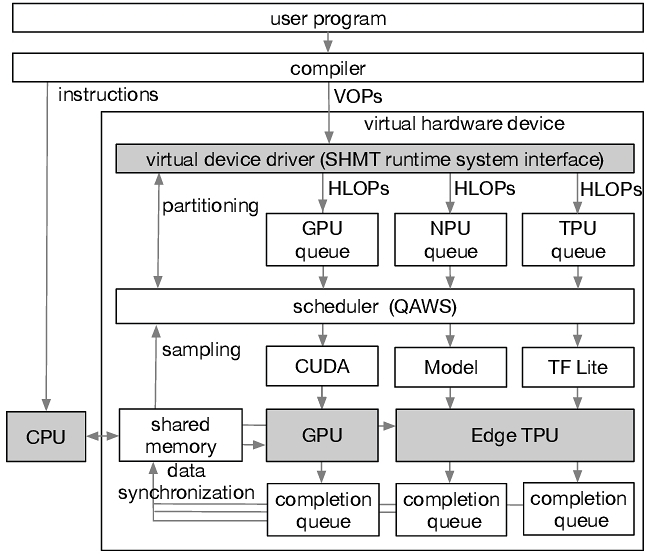
\includegraphics{micro23-41-fig3.jpg}
    \caption{SHMT overview}
    \label{fig:enter-label}
\end{figure}

Para lidar com tais desafios na implementação do SHMT, o texto propõe uma arquitetura de sistemas, abstraída na forma de um dispositivo/hardware virtual, conforme a figura 1, implementado como loadable kernel module (LKM) e com os seguintes componentes:

\begin{itemize}
  \item \textbf{Virtual Operations (VOPs) and High-Level Operations (HLOPs):} VOPs e HLOPs são conjuntos de operações/interface com a finalidade de prover ao compilador ou aos usuários funcionalidades suportadas pelo SHMT, e definir como o SHMT interage com os hardwares disponíveis a ele.

As VOPs ajudam a abstrair todo o subsistema SHMT como um acelerador único da perspectiva do software usuário, que interage com o SHMT por meio delas. Para este trabalho, os autores implementaram VOPs de modo a atender as funcionalidades mais recorrentes em aceleradores, como convolução e redução de soma, e apresentam operações tanto element-wise como tile-wise matrix.

Por outro lado, uma HLOP define um subconjunto de ações de uma operação VOP que um dispositivo de computação pode suportar. Uma HLOP também define a granularidade e o tipo dos dados que um acelerador pode suportar, ao contrário de uma VOP, que não possui restrição nos tamanhos dos dados de entrada/saída. Para cada VOP, o runtime system do SHMT particionará dinamicamente o trabalho e os dados em HLOPs e atribuirá cada HLOP para um acelerador, tendo em vista os tamanhos de dados e o modelo de paralelização aplicado.
  
  \item \textbf{Runtime system do SHMT:} Para cada VOP que o SHMT recebe, o runtime system, implementado como driver do hardware virtual, descobre os recursos de hardware disponíveis para executar a VOP, coleta informações sobre o método de paralelização e particionamento dos dados e consulta o escalonador, que de acordo com sua política, mapeia as tarefas a recursos de hardware. Com um plano sugerido pelo escalonador, o runtime system realiza o particionamento da VOP em HLOPs, para os aceleradores, nos tamanhos de dados suportados por eles e então atribui as HLOPs às filas de entrada de cada dispositivo. Cada fila possui uma thread monitorando, cuja uma das responsabilidades é executar as HLOPs da fila sempre que o dispositivo alvo estiver disponível. Uma vez que uma HLOP termina, a thread moverá a tarefa para uma fila de conclusão que o runtime system do SHMT pode posteriormente retirar e usar para fins de agregação de dados e sincronização.
  
  \item \textbf{Quality-Aware Work-Stealing (QAWS) Policy:} A política de QAWS tem como objetivo garantir qualidade das regiões de dados críticas, enquanto mantém um overhead baixo no escalonamento de tarefas. Para cada partição de dados de entrada, o QAWS amostra os dados para determinar a criticidade e atribui a carga de trabalho a um hardware de acordo com ela. No artigo são examinadas duas políticas, que resumidamente são: Device-dependent limit, na qual cada dispositivo de processamento tem um conjunto de limitações de hardware aceitáveis baseado em sua precisão de dados e acurácia, de modo que o QAWS atribui aos aceleradores dados menores do que seus limites de criticidade, e permite que esses dispositivos roubem HLOPs de outros, com o mesmo, ou menores limitações de hardware; Application-dependent top-K\%, política que ranqueia a criticidade dentro de uma janela de partição de dados e escalona top-K\% das partições ao hardware de maior acurácia, o top-S\% ao segundo de hardware de maior acurácia e assim por diante. Nessa política, os valores de K e S devem ser fornecidos pela aplicação, por meio de uma VOP, indicando a porcentagem de dados que geralmente são críticos. Também com o seu uso é apenas permitido roubo de HLOPs/tarefas de um dispositivo por outro de maior acurácia.

Para determinar a criticidade de uma partição de dados, o SHMT usa a técnica conhecida como input responsiveness approximation (IRA), tendo em vista duas métricas, intervalo de dados (ou seja, valores máximo e mínimo) e desvio padrão dentro da região. O texto propõe e testa experimentalmente também 3 métodos de amostragem: striding, random e reduction.
\end{itemize}

\section{Resultados Apresentados}
Para a execução dos testes, foi usada uma máquina protótipo customizada com uma Jetson Nano da NVIDIA e uma Edge TPU comercial da Google. O módulo Jetson Nano contém um processador quad-core ARM A57 e 128 núcleos de GPU Maxwell. Uma Edge TPU foi conectada ao sistema através do slot m.2 na parte de trás do módulo Jetson Nano. Os três tipos de unidades de processamento, CPU, GPU e Edge TPU, trocam dados através da interface PCIe embarcada. O sistema protótipo contém uma interface LPDDR4 de 64 bits com 4 GB a 25,6 GB/s como memória principal. A memória principal do sistema hospeda os dados compartilhados entre CPU, GPU e Edge TPU. A Edge TPU adicionalmente contém 8 MB de memória do dispositivo. O sistema montado roda um Ubuntu Linux 18.04 com o kernel personalizado 4.9.253-tegra da NVIDIA. Os escritores relatam que nesse ambiente a Edge TPU pode assumir o papel de um acelerador de funções matriciais ou de uma NPU.


A fim de realizar benchmarks, foram utilizadas aplicações de repositórios públicos com o objetivo de cobrir diferentes domínios de aplicação, tais como processamento de imagens, processamento de sinal, simulações físicas e finanças. Com essas aplicações, diferentes políticas de escalonamento e referências/baselines , foram analisados o speedup de latência fim-a-fim, qualidade das políticas QAWS, consumo de energia, uso de memória e overhead de comunicação.

Ao comparar a latência fim-a-fim do SHMT a uma implementação de GPU otimizada, o SHMT com a política QAWS Top-k\% e amostragem do tipo striding, que se mostrou a mais performática nos experimentos, obteve um speedup médio de 1.95x. Durante a análise dos dados de latência, os escritores enfatizam que o uso de políticas QAWS Top-k\%, mesmo que com diferentes tipos de coleta de amostras, mostrou-se mais adequado para o escalonamento de cargas de trabalho de desempenho crítico, atribuindo essa performance à possibilidade de Edge TPUs trabalharem em algumas partições de dados com faixas de valores ou variações mais amplas do que a política Device-dependent limit. Como comparação, também foram analisadas 2 políticas que não preocupam-se com a qualidade de dados, distribuição igual dos dados e work-stealing, além de uma implementação de GPU com software pipeline, que respectivamente possuem o speedup médio de 0.98x, 2.07x e 1.27x. Observa-se no trabalho que a distribuição igualitária dos dados tem a performance limitada pelo hardware de menor desempenho, enquanto que o work-stealing permite que hardware de melhor desempenho realize mais tarefas. O texto conclui então, que a política de work-stealing é a mais performática e diverge da QAWS de melhor desempenho devido ao overhead de amostragem dos dados.

Com objetivo de atestar a qualidade dos dados gerados pelo SHMT com as políticas QAWS, foram utilizadas duas métricas, Mean Absolute Percentage Error (MAPE) e Structural Similarity Index Measure (SSIM), além de usar como referência um cenário oráculo, no qual todas as regiões críticas a serem processadas foram identificadas e atribuídas a HLOPs manualmente. Observou-se então que o MAPE médio, ao executar diferentes aplicações, do cenário oráculo é de 1.77\%, enquanto que o SHMT com work-stealing é de 2.85\% e ao adotar políticas QAWS o MAPE de todas as variações de políticas não ultrapassou 2\%, implicando que um overhead de amostragem é overkill para a maior parte dos casos. Devido a variações significativas dos valores de MAPEs entre as aplicações, tendo picos principalmente naquelas com foco em processamento de imagem, os escritores analisaram o SSIM como uma métrica adicional, observando o valor de 0.9957 para o cenário oráculo e valores acima de 0.97 para o SHMT ao usar todas as variações da política de QWAS, atestando novamente que não é preciso um grande overhead na amostragem dos dados.

Os escritores acreditam que ao reduzir o tempo total de execução e realizar offloading de tarefas para uma Edge TPU com baixo consumo de energia, o SHMT tem um grande potencial de economia energética. Eles alegam, ao analisarem o consumo de energia de GPUs e do SHMT (com a QAWS top-k\% e amostragem striding) em diferentes aplicações, uma redução média no consumo de 51.0\% por parte do SHMT e respectivamente uma potência de pico de 4.67 watts e 5.23 watts. Atribuem essa redução ao speedup de 1.95\% que reduz o período de consumo, com 5.23 watt no pico.

Tendo como baseline GPUs, também é discutido nos resultados a pegada de memória do sistema descrito. Constata-se que a lógica especializada nos Edge TPUs oferece mais funções aceleradas em hardware, de modo que é necessário menos memória do sistema em comparação com implementações equivalentes em GPUs. É dito que isso ocorre porque os buffers nos elementos de processamento do Edge TPU podem substituir a memória usada para armazenar os resultados intermediários de produtos vetoriais, resultando em uma redução na pegada da memória do SHMT para aplicações com quantidades significativas de HLOPs nos Edge TPUs, apesar da inclusão de buffers adicionais para entradas nos Edge TPUs.

 É relatado também que os dispositivos de computação no SHMT gastam apenas cerca de 1\% ou menos do tempo esperando por trocas de dados, por várias razões. Primeiro, o modelo de programação paralela do SHMT promove algoritmos de paralelismo de dados, que implicitamente têm baixas trocas de dados entre blocos paralelos de computação. Segundo, o tempo de computação é relativamente mais longo em cada processador do que o tempo de troca de dados, permitindo mecanismos como o de duplo buffering para ocultar a latência. Terceiro, a quantidade de HLOPs de cada aplicativo permite que o sistema de tempo de execução do SHMT supra os recursos de processamento disponíveis e cubra a latência da troca de dados.

\section{Analíse do artigo}

O uso de unidades de processamento especializadas, também conhecidas como aceleradores, tornou-se padrão nos tempos atuais. Hoje, observamos esses módulos sendo empregados principalmente em áreas como Machine Learning/Inteligência Artificial, jogos e realidade aumentada, nas quais é exigido desempenho que uma CPU de uso geral não pode oferecer. Esse cenário produziu sistemas de computação heterogêneos empregados tanto em wearables e smartphones quanto em computadores pessoais e clusters HPC. No entanto, os frameworks de programação convencionais, incluindo linguagens de domínio específico, geralmente delegam regiões de código exclusivamente a um tipo de processador, deixando outros recursos de computação ociosos sem contribuir para a função executada.

O trabalho relatado propõe então o SHMT, um modelo que pode utilizar esses diferentes tipos de unidades de processamento concorrentemente na execução de uma mesma região de código, teoricamente aumentando o throughput, diminuindo a latência de tarefas e reduzindo o consumo de energia, caso as unidades de processamento tenham desempenho similar. Tais ganhos teóricos são atingidos no trabalho discutido, o SHMT, ao permitir, através de suas VOPs e HLOps, a execução de Kernels em diferentes tipos de aceleradores, tratando a transferência/sincronização dos dados e garantindo uma boa qualidade dos resultados, com baixo overhead de escalonamento, ao usar suas políticas QWAS, entrega a seus usuários um speedup médio de 1,95X e uma redução média no consumo de energia de 51,0\%, tendo como baseline o uso de GPUs.

Soluções de distribuição de tarefas existentes para sistemas heterogêneos que utilizam vários aceleradores costumam empregar os seguintes métodos. (1) Particionamento de uma aplicação e mapeamento das partições em múltiplos aceleradores do mesmo tipo (como GPUs) no sistema de computador para execução simultânea. Embora esses métodos possam alcançar um desempenho mais alto com a execução paralela de vários dispositivos do mesmo tipo, eles não consideram o uso simultâneo de outros tipos de aceleradores heterogêneos no mesmo sistema, como o SHMT faz. (2) Estendendo o método (1) para múltiplos aceleradores com diferentes configurações ou versões, mas ainda do mesmo tipo. Trabalhos que utilizam este método novamente não lidam com os desafios de utilizar simultaneamente diferentes hardwares. (3) Permitindo o uso concorrente de vários tipos de aceleradores apenas quando a execução da tarefa dispara várias funções dedicadas ao mesmo tempo. No entanto, o comportamento do fluxo de execução do programa e as diversas características das funções dedicadas que mapeiam para domínios específicos podem limitar o nível de execução simultânea e heterogênea. Enquanto o SHMT fornece um modelo de programação independente de máquina para partições de tarefas, permitindo um maior aproveitamento de hardware e uma aplicabilidade mais ampla para aceleradores.

Por fim, torna-se evidente que a adoção de modelos de computação como o SHMT pode proporcionar ganhos significativos de desempenho para os sistemas heterogêneos modernos. Isso se deve à arquitetura diferenciada do SHMT, capaz de lidar com a heterogeneidade dos processadores que compõem um sistema. Essa capacidade permite o uso simultâneo desses componentes, explorando ao máximo o nível de paralelização do hardware disponível, sem comprometer a precisão dos resultados obtidos. Esse alto nível de paralelismo resulta na redução do consumo de energia e em um desempenho superior no processamento de tarefas, quando comparado aos modelos tradicionais de paralelização.
\end{document}
